
\documentclass[journal]{IEEEtran}
\usepackage[utf8]{inputenc}
\usepackage{cite}
\usepackage[cmex10]{amsmath}
\interdisplaylinepenalty=2500
\usepackage{algorithmic}
\usepackage{array}
\usepackage{url}
\hyphenation{op-tical net-works semi-conduc-tor method methods}

\ifCLASSOPTIONcompsoc
  \usepackage[caption=false,font=normalsize,labelfont=sf,textfont=sf]{subfig}
\else
  \usepackage[caption=false,font=footnotesize]{subfig}
\fi

\ifCLASSINFOpdf
  \usepackage[pdftex]{graphicx}
  % declare the path(s) where your graphic files are
  % \graphicspath{{../pdf/}{../jpeg/}}
  % and their extensions so you won't have to specify these with
  % every instance of \includegraphics
  \DeclareGraphicsExtensions{.pdf,.jpeg,.jpg,.png}
\else
  % or other class option (dvipsone, dvipdf, if not using dvips). graphicx
  % will default to the driver specified in the system graphics.cfg if no
  % driver is specified.
  \usepackage[dvips]{graphicx}
  % declare the path(s) where your graphic files are
  % \graphicspath{{../eps/}}
  % and their extensions so you won't have to specify these with
  % every instance of \includegraphics
  \DeclareGraphicsExtensions{.eps}
\fi

%opening
\title{A Simulator for Event-oriented Data in Flexible Assembly System Fault Prediction - DRAFT}
\author{Tero Keski-Valkama}

\begin{document}

\maketitle
Version: \today

\begin{abstract}

\end{abstract}

\begin{IEEEkeywords}
\end{IEEEkeywords}

\section{Introduction}
This paper describes a method for simulating event-oriented data sources of a flexible assembly system including faults. Such simulator is required for creating representative corpuses
of data for teaching automated learning algorithms for predictive maintenance and systemic fault detection.

Flexible assembly system was described by Donath and Graves \cite{donath1988flexible} as a system consisting of a set of products each with a specified volume
assembled on a workshop consisting of a fixed number of cells. In practise, a flexible assembly system contains parts and materials stored in an intermediate storage,
a conveyor or crane system to move the parts, materials, intermediate assemblies and finished products between the cells, and the cells with work machines and necessary tooling
to assemble and process intermediate assemblies and products. The cells might consist of for example manual assembly steps, robotic assembly cells, CNC lathes, or 3D printing.

As opposed to more specialized industrial production systems, flexible assembly systems are designed for smaller batches and greater flexibility so that the set of end products can vary more widely.
For example, flexible assembly systems can be reconfigured more conveniently following the evolution of new versions of the end products. Flexibly assembly systems also allow for a wider range
of customization between the different end product instances of the same product. The nature of fast evolution of configurations and workflows, and heterogeneous operating conditions make
planning maintenance more challenging.

System downtime is a significant cost for flexible assembly systems. System downtime is reduced by preventive maintenance typically scheduled periodically.
Recently Internet of Things and opening of the networked industrial system APIs have created new possibilities for predictive maintenance and systemic fault detection. Different sites with similar
flexible automation systems have widely different environmental and workload conditions which has an impact on the wear and tear of the flexible automation system components.
Taking different site environments and workloads into account when planning preventive maintenance cycles is non-trivial. There is a clear need to adapt maintenance based on actual
conditions in the operation rather than by simply scheduling maintenance periodically. It is also important to indicate potential faults early to improve the response time of corrective action.

Going from preventive maintenance towards predictive maintenance optimizes and targets the maintenance related costs towards the activities that have best impact
on improving the availability and operation of deployed flexible manufacturing systems.
Predictive maintenance in flexible assembly systems benefits from automatic indicators for potential future faults.
Current predictive maintenance systems concentrate on measuring device health for example by means of measuring temperature and vibration
\cite{contreras2002integrating}. Less research effort is done in the context of event-oriented data sources (logs), and about systemic failures.

Evaluating novel automatic methods for fault prediction requires standard benchmarks to compare these methods against. Currently there are no standard benchmarks to test
different anomaly detection methods and compare their performance against each other. Such standard benchmarks exist in other fields of machine learning,
such as the MNIST handwritten digits benchmark\cite{lecun-mnisthandwrittendigit-2010}. Realistic simulations are often used\cite{jager2014assessing} for domains where
real data is hard to collect or where real data would be subject to business confidentiality. Training neural network and other learning systems often utilizes realistic
simulations instead of real data. Real measured data is often limited in both state space and in volume, and often simulations give better results \cite{duch2005artificial}.

Fault-free simulations of flexible assembly systems are generally available\cite{giulio} and have been studied for visualization and optimization purposes.
These are not directly suitable for benchmarking fault detection methods.

\section{Problem Formulation}

A standard benchmark should reflect a realistic task and it should have enough data to be useful.

Real data regarding flexible assembly system faults is
not generally available, because fault data is generally subject to business confidentiality in flexible assembly industry.
The generally available simulation models do not typically contain failure modes and are not typically designed to emit
log structured events in a realistic fashion, but they can be used as a starting point in creating a flexible assembly system model.

To enable relevant research into anomaly detection in flexible assembly systems a realistic simulator for logged events is needed.
All references to simulated faults and failure modes in the research described in this article are hypothetical and should not be considered to
reflect actual characteristics of any specific existing systems. An effort is made to make the simulations contain the necessary features of
generic and realistic failure modes to make the models useful for research, but for example the simulated fault frequencies and the configuration
of the flexible assembly system along with workflows and end products are arbitrary and hypothetical.

A simulation for benchmarking anomaly and fault detection methods should not be fully deterministic to reflect the real world dynamics. The simulation should also
include realistic faults with possible early indicators such as variations in delays in the steps of the process. The focus of the simulator is on faults without pre-existing
diagnostic fault codes, such as unexpected faults and degradation of the assembly modules and conveyors, and on systemic faults. Systemic faults in this paper
mean faults and degradation of output where each of the component modules of the Flexible Assembly System are seemingly operating without faults.

\section{Modes of Failures in Flexible Assembly Systems}

Flexible assembly system failures are typically component failures where a failure of a single module or a component will lead to the system becoming inoperational.
Since the flexible assembly systems are dynamic systems with numerous moving parts, the wear and tear of the components and tools are a significant source of downtime.
In addition to the component failures, certain systemic failures can cause downtime, such as power loss and network communication failures.
The critical systemic failures mentioned don't typically show any indication before they happen so predictive maintenance has little potential to be applied there.
In addition to these critical system failures,
the whole system can exhibit modes of failure and degradation which are not directly attributable to single component degradation or failure. Some of these might be caused by
external factors, such as accidents and human errors, but also for example by timing issues in the whole process causing unexpected queues or traffic jams.

Tool wear and tear depends on the workload. Typically tools that wear out fast, for example multiple times for one unit of work in a cell, receive much attention and such tools are generally
well maintained. Tools that have wear and tear but have longer life spans are more susceptible to being overlooked by operators and might have some indicators of degrading
before a failure. Cranes, hatches and conveyors have relatively long life spans and are primarily maintained in periodic preventive maintenance. If we could get indicators
for impending failure for these components, the periodical maintenance could be scheduled earlier to prevent downtime. In addition to these physical faults the flexible
assembly system can suffer from human errors. Human operator can inadvertently misconfigure the flexible assembly system so that its operating mode changes unexpectedly,
for example by disabling a cell which can lead to the system stopping without a proper failure. In addition to configuration
errors, human operators might fail in manual assembly steps for example by pressing the button to mark the step
as completed too quickly.
The flexible assembly system might also get in incompatible materials, parts or replacement tools and fail when trying to use them.

There has lately been an increase of computer crime against industrial networks as the devices and systems become more connected.
Nation states execute industrial espionage and even sabotage against each other\cite{stuxnet}. An electronic sabotage attack might present itself
much like a human misconfiguration error, and would be potentially detected in a similar fashion even if the attack itself would not be
directly visible in the logs as anomalous activity.

For useful anomaly detection systems we need to concentrate on faults that are unexpected without pre-existing diagnostic error codes, and that potentially have early indications
in collected event-based logs. Early indication in this context means that the error can be detected in the system logs before the failure becomes otherwise evident.
The table \ref{faults} summarizes the classes of faults.

\begin{table}[!t]
\renewcommand{\arraystretch}{1.3}
\caption{Table of recognized fault types in flexible assembly systems}
\label{faults}
\centering
\begin{tabular}{|p{25mm}|p{15mm}|p{15mm}|p{15mm}|}
\hline
Fault type & Unexpected faults & Potentially has an early indication & Useful target for anomaly detection \\
\hline
\hline
Auxilliary component wear and tear & X & X & X \\
\hline
Critical systemic failures (power, network) & X & & \\
\hline
Human error, failed manual step & X & X & X \\
\hline
Incompatible parts, materials or replacement tools & X & & \\
\hline
Systemic failures (jams, accidents, misconfigurations, cyberattacks) & X & X & X \\
\hline
Tool wear and tear for quickly degrading tools & & X & \\
\hline
Tool wear and tear for slowly degrading tools & X & X & X \\
\hline
\end{tabular}
\end{table}

\section{Flexible Assembly System Model}

The simulation consists of a realistic model of a flexible assembly system with a class of faults randomly injected into the process.
The simulation will not be fully deterministic and contains soft faults which do not affect operation in addition to hard faults which result in immediate downtime.

The simulator is implemented in Python and it generates a JSON file which models the logs from the system. The log message fields are defined in Table \ref{fields} and
and example message is shown in \ref{samplemessage}.

The simulation framework consists of a scheduler that takes the next event from the event queue and applies it to the respective module. The simulated modules
execute when events are applied to them and generate new events and immediate log entries with timestamps and other metadata.
The simulated modules have optional active failure modes that affect the simulated operation of the component through
generated log messages or the subsequent generated events. Failure modes are set up to the simulated modules in a separate failure module.
The overall framework sets up the simulation and events.

\subsection{Normal Operation of the Simulated System}
The simulated hypothetical system assembles and tools a car transmission block loosely inspired by a Youtube video of Chrysler transmission assembly\cite{transmission}.
The workflow consists of several manual assembly steps in separate cells and transporting the subassemblies between the cells by the means of
cranes and conveyors. Multiple transmission blocks are being assembled simultaneously in separate cells.

The transmission component consists of four subassemblies. The main sequence starts from the frame of the transmission block
and continues through several manual steps done in separate cells. The steps of the main sequence are given in
the Tables \ref{mainsteps1} and \ref{mainsteps2}.
Each step can contain a separate sequence of events and associated log messages.
The mean durations for manual steps can vary in normal operation $\pm$ thirty percent. The mean durations for automatic steps can vary
$\pm$ five percent.

The production frequency of the transmission blocks depends on the slowest step as in this case there is only one cell for one step and no
parallel work is possible within one step. The slowest step takes about 76 seconds. In this hypothetical assembly plant, new transmission block
frames are added every 100 seconds and the final transmission blocks are being produced roughly in the same interval. This means that there
will be at maximum roughly seven transmission blocks in different stages being produced at the same time.

\begin{table}[!t]
\renewcommand{\arraystretch}{1.3}
\caption{Table of the steps 1-16 in the main assembly process}
\label{mainsteps1}
\centering
\begin{tabular}{|p{5mm}|p{20mm}|p{10mm}|p{15mm}|p{15mm}|}
\hline
Step & Description & Duration & Log messages & Potential failures \\
\hline
\hline
1 & Crane & 30 s & Going forward, stopping, going back, stopping & Wear \& tear \\
\hline
2 & Manual inspection & 37 s & OK pressed & Failed manual step \\
\hline
3 & Conveyor & 30 s & To cell, stop, to next cell & Wear \& tear \\
\hline
4 & Bowl feeder gives components & 5 s & Given & Wear \& tear \\
\hline
5 & Add components & 21 s & OK pressed & Failed manual step \\
\hline
6 & Conveyor & 30 s & To cell, stop, to next cell & Wear \& tear \\
\hline
7 & Bowl feeder gives components & 10 s & Given & Wear \& tear \\
\hline
8 & Add components & 34 s & OK pressed & Failed manual step \\
\hline
9 & Conveyor & 30 s & To cell, stop, to next cell & Wear \& tear \\
\hline
10 & Crane with subassembly A & 10 s & Going forward, stopping, going back, stopping & Wear \& tear \\
\hline
11 & Combine with subassembly A & 34 s & OK pressed & Failed manual step \\
\hline
12 & Conveyor & 30 s & To cell, stop, to next cell & Wear \& tear \\
\hline
13 & Conveyor with subassembly B & 10 s & To cell, stop & Wear \& tear \\
\hline
14 & Combine with subassembly B & 35 s & OK pressed & Failed manual step \\
\hline
15 & Conveyor & 30 s & To cell, stop, to next cell & Wear \& tear \\
\hline
16 & Bowl feeder gives components & 5 s & Given & Wear \& tear \\
\hline
\end{tabular}
\end{table}

\begin{table}[!t]
\renewcommand{\arraystretch}{1.3}
\caption{Table of the steps 17-31 in the main assembly process}
\label{mainsteps2}
\centering
\begin{tabular}{|p{5mm}|p{20mm}|p{10mm}|p{15mm}|p{15mm}|}
\hline
Step & Description & Duration & Log messages & Potential failures \\
\hline
\hline
17 & Conveyor with cover & 10 s & To cell, stop & Wear \& tear \\
\hline
18 & Add cover and bolts & 76 s & OK pressed & Failed manual step \\
\hline
19 & Conveyor & 30 s & To cell, stop, to next cell & Wear \& tear \\
\hline
20 & Tighten the bolts & 28 s & OK pressed & Failed manual step \\
\hline
21 & Conveyor & 30 s & To cell, stop, to next cell & Wear \& tear \\
\hline
22 & Conveyor with subassembly C & 10 s & To cell, stop & Wear \& tear \\
\hline
23 & Combine with subassembly C & 60 s & OK pressed & Failed manual step \\
\hline
24 & Conveyor & 21 s & To cell, stop, to next cell & Wear \& tear \\
\hline
25 & Tighten the bolts & 16 s & OK pressed & Failed manual step \\
\hline
26 & Conveyor & 21 s & To cell, stop, to next cell & Wear \& tear \\
\hline
27 & Bowl feeder gives components & 5 s & Given & Wear \& tear \\
\hline
28 & Add components & 11 s & OK pressed & Failed manual step \\
\hline
29 & Conveyor & 21 s & To cell, stop, to next cell & Wear \& tear \\
\hline
30 & Tighten the bolts & 32 s & OK pressed & Failed manual step \\
\hline
31 & Conveyor & 21 s & To output gate & Wear \& tear \\
\hline
\end{tabular}
\end{table}

\subsection{Simulated Failure Modes}
It is regrettable that real data on faults in real flexible assembly systems are not available, but in any case it is possible to make reasonable
models based on existing data from other analogous sources such as \cite{nasaames} and \cite{tsarouhas2009classification}.

The previous subsection describes the normal operation of the system. The failure modes of the manual steps include human errors by pressing OK
prematurely without properly executing the step. This leads to the next manual step failing and returning the block back to the previous step or
removing it from the assembly line altogether. Misconfiguration can cause different kinds of results, but here we assume some work step is skipped
so that it is not noticed and doesn't directly prevent other steps from being executed. Failed manual steps also include wear and tear
on the tools which gradually increases the duration of the work before causing a fault. The human operator can also tire and lose concentration
when doing lots of repetitive steps. There are studies showing how speed performance degrades in general in a linear fashion in humans
under fatigue and boredom, for example\cite{fatigue}. Switching human operators during the day might change the effective performance slightly.

The automatic steps wear and tear cause gradually increasing durations for the step also until at some point the step stops functioning and
intermediate assemblies start piling up until a fault is signalled because of exceeding the limits of intermediate storage space.

Duration increases before a fault are non-deterministic and for some faults they don't actually happen before the fault. The profile of the duration
increase depends on the type of device used for the step. Generally mechanical wear and tear effect on machine health profile follows
an accelerating curve downwards \cite{eker2012major}, \cite{milldataset}. For the purposes of simulation I assume machine health has an approximately
linear effect on machine performance measured in delays and success rates in applicable types of faults.

Simulated wear and tear causes two types of delay profiles. First,
a continuous wear and tear typically causes no measurable delays at first, but when the degradation accumulates the delay increases following
a roughly exponential curve \ref{continuouswearandtear}. Second, for certain steps, such as taking bolts from the bowl feeder a human operator
might fail to grab a bolt from time to time. Typically human operator tries again and succeeds. The frequency of the failure increases
slowly and roughly following an exponential curve until the failure rate becomes apparent and causes the operator to take corrective action,
typically causing downtime. These failures cause a random delay if they happen. This characteristic delay profile is depicted in \ref{retrydelays}.

While the directly visible fault modes are easier to model and characterise, complex flexible assembly systems also have warnings and trace messages
which are signalled into logs, but are not signalled to operators in real time because most of the time these messages are not a cause for concern.
An example of such a signal could be for example a health warning of a device that happens spuriously once every now and then for normal operation,
but increases in frequency when the device actually starts to fail. There can also be log messages for example for electrical switches turning
on and off when the working step is active, but never while the step is not active. Anomalies in such messages are an indicator of potential
future fault.

In addition to unexpected component failures, we have to simulate systemic failures. The simulated systemic failures and their effects are listed in the table \ref{systemicfailures}.

\begin{table}[!t]
\renewcommand{\arraystretch}{1.3}
\caption{Table of the steps 1-16 in the main assembly process}
\label{systemicfailures}
\centering
\begin{tabular}{|p{20mm}|p{20mm}|p{20mm}|}
\hline
Failure & Description & Effect \\
\hline
\hline
Accident & TODO  & TODO \\
\hline
Cyberattack & TODO  & TODO \\
\hline
Jam & TODO  & TODO \\
\hline
Misconfiguration & TODO  & TODO \\
\hline
\end{tabular}
\end{table}

\section{Implementation}

The FAS Simulator\cite{FASSimulator} is implemented in Python as a discrete event simulator. Each step of the assembly process is an actor which receives and generates
delayed events in model time. Each step of the assembly process manages its own internal state, and possible failure modes.

The example simulation consists of stereotypical models of the steps of the process with input signals and configurable output signals. For example, simulating
the operation of a crane an instance of a module named Crane is configured and added to the respective position in the process in relation to other module instances.
The Crane module maintains an internal queue of items to transport, and generates delayed output events for each of the input event in sequence, so that only one item is
transported at a time. This is in contrast to conveyor module instances which don't have an internal queue, as the conveyors transport the items independently and in parallel.

The simulation is set up by first defining the topology of the process by instantiating the respective modules and configuring their bindings to other modules. The actual simulation
is done simply by triggering the global process inputs as required, causing sequences of events being generated accordingly.

The events are logged in JSON with a timestamp and an event type, resembling logs in a real Flexible Assembly System.

The simulator in principle allows defining different kinds of discrete event simulators. Several specific types of simulations are pre-defined for the purposes of benchmarking
different modelling approaches. These pre-defined simulations vary in complexity and length from trivial one item at a time sequences to complex multiple items at once simulations.
Each type of simulation can also be configured to fail in specific ways to test different failure detection approaches. All the simulations are based on the Flexible Assembly System
defined in this article and the simulations are stochastic in respect to delays between steps.

\section{Evaluation}

The FAS Simulator is evaluated by testing several methods for inferring the hidden process behind the event sequences and existing methods of fault detection for
the event sequences.
The simulation is considered useful if it can be reasonably expected to mirror the real world contingencies and patterns, and if it is not completely trivial to
learn or infer by existing methods. If the simulator creates event sequences that are challenging to learn by existing methods, then it is useful as a benchmark
in relation to improving those methods and in creating new ones.

For the purposes of this article, we will only consider methods which are not trained based on known error conditions beforehand. Thus, the failure prediction challenge
becomes a challenge of learning the correct operation of the system and flagging any inconsistencies and anomalies.

For evaluation purposes, we will use a generated fault-free event sequence with first one complete sequence for one item only, then for 20 items simultaneously going through the system,
and finally 50 items being assembled in the system simultaneously in the same log file. This results in a log file with a sequence of 2627 ($ = 37 \cdot 31 $) events of 35 different
event types. A depiction of the simulated event sequence is shown in the Figure \ref{figure:events}. The first item goes through the process alone, so the events on the left side
of the graph are in perfect, deterministic order from the bottom to the top. However, for multiple parallel items being processed it becomes evident that the previous event doesn't in itself
completely determine the next event. This indeterminate order of sequential events is shown in a zoomed portion of the graph in the Figure \ref{figure:zoomed_events}
Some queue effects are also visible in the later parts of the sequences.

\begin{figure}[tb]
 \centering
 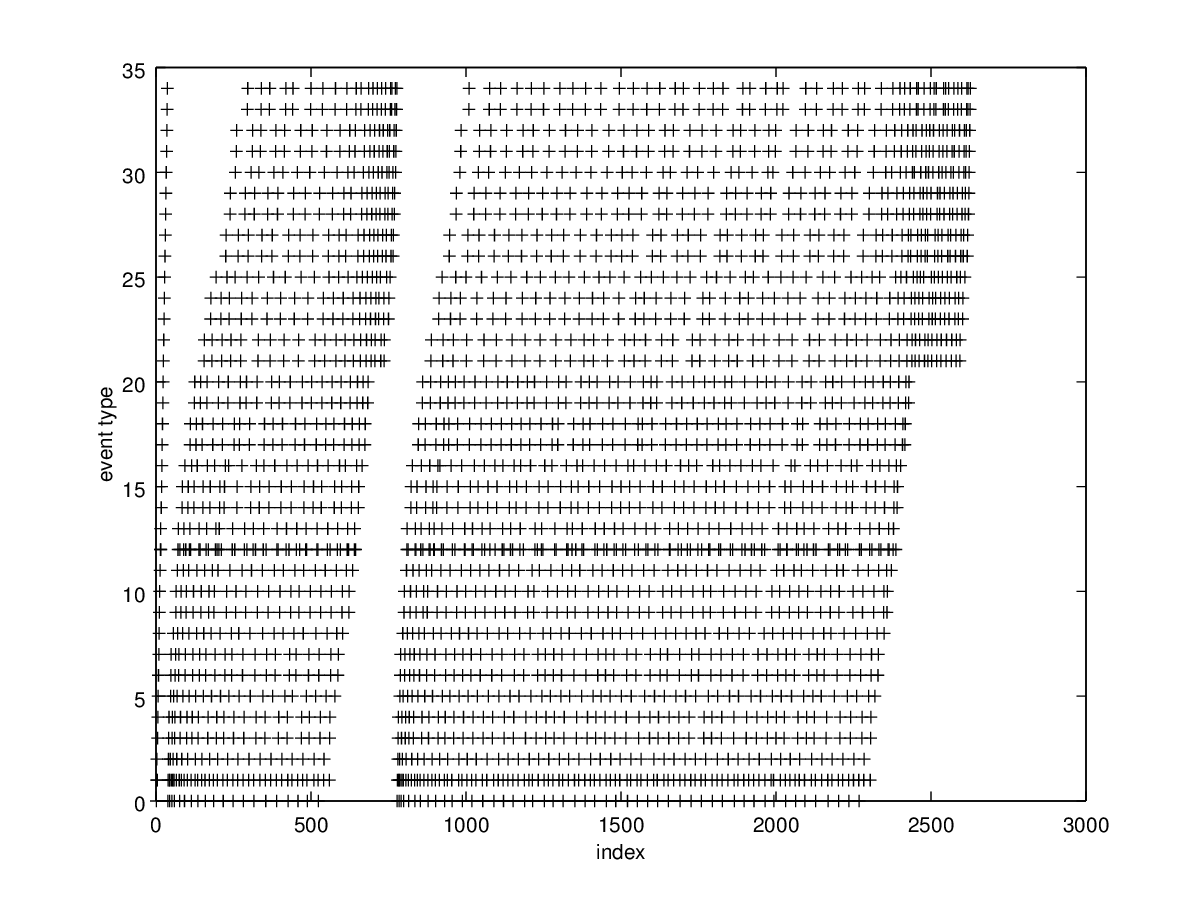
\includegraphics[width=8 cm,keepaspectratio=true]{./events.png}
 \caption{A representative log of event types graphed against time}
 \label{figure:events}
\end{figure}

\begin{figure}[tb]
 \centering
 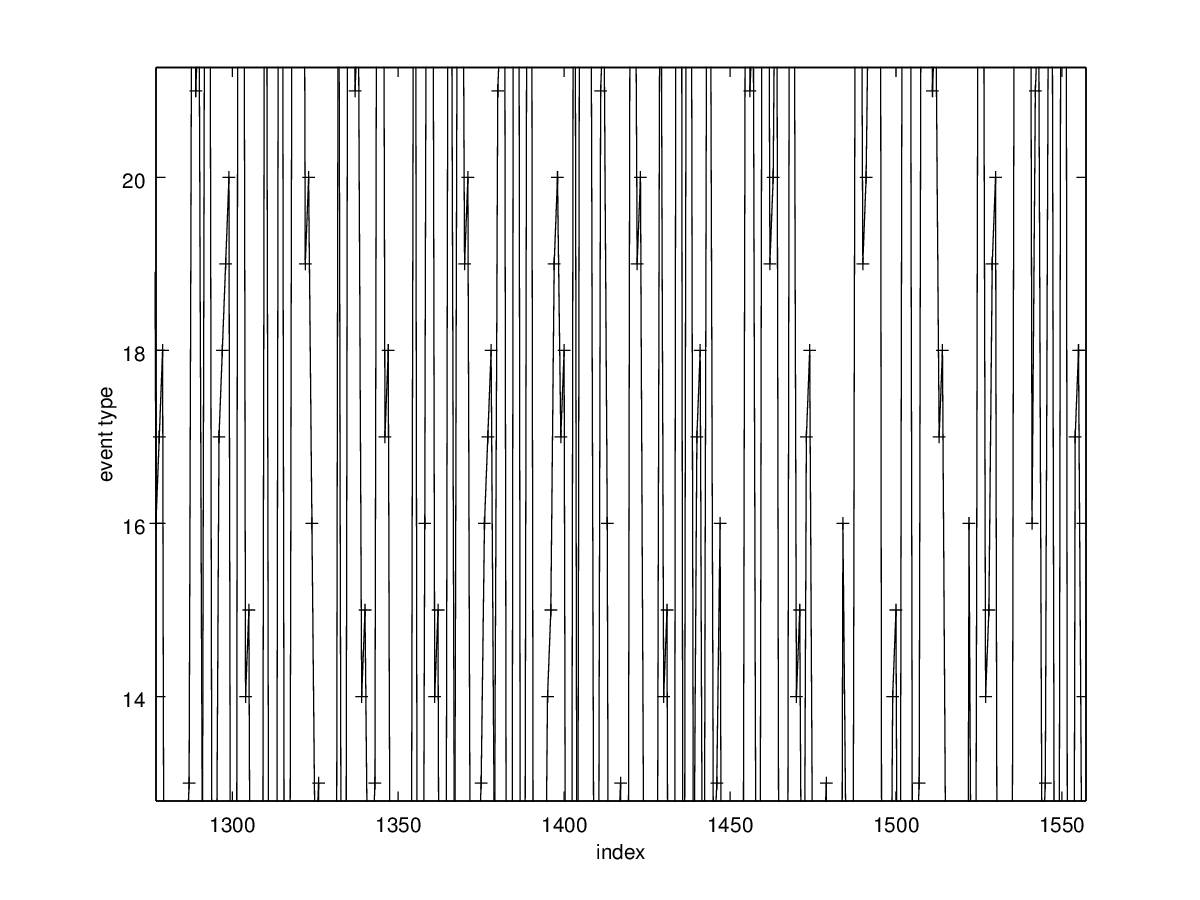
\includegraphics[width=8 cm,keepaspectratio=true]{./zoomed_events.png}
 \caption{A detail of the graphed log of events. The lines connect the events in sequence, showing the indeterministic order}
 \label{figure:zoomed_events}
\end{figure}

\section{Results}

A trivial DFA model from interpreting all the observed events as both transitions and states is depicted in the Figure \ref{figure:trivial_DFA}.
This DFA accepts any sequence consisting of transitions between any two events observed in the training data. The trivial DFA cannot be minimized by Moore minimization,
as there are no two states with exactly the same outwards transitions at least in the training sequence tested.
It is evident that because of parallel processing of multiple items in the FAS System, almost any state transition is
in practice possible even in fault-free sequences, but some didn't happen in the training data.
The trivial DFA model is incapable of inferring higher level patterns from the sequences, and would simultaneously make a great number of false positive
and false negative errors.
\begin{figure}[tb]
 \centering
 \includegraphics[width=8 cm,keepaspectratio=true]{./dfa.png}
 % dfa.png: 9992x3323 pixel, 72dpi, 352.50x117.23 cm, bb=0 0 9992 3323
 \caption{A trivial DFA interpreting the events as both the states and the transitions}
 \label{figure:trivial_DFA}
\end{figure}

The second baseline benchmark is done by automatically inferring a deterministic finite automaton from the fault-free log events using Angluin learner (L*)\cite{Angluin},
following the description by Langer et al.\cite{langer2011self}. Langer showed that Angluin learner was able to learn small toy examples very well, but didn't work very well
for a real world example of a stream of events recorded from a CAN bus of the powertrain network of an electric vehicle.

\section{Conclusion}

This study presents a benchmark model for validating anomaly detection methods for flexible assembly systems using log structured data.
Existing systems for predictive maintenance concentrate on measuring health of a separate devices based on typical degradation characteristics
for such devices. They also concentrate on continuous measurement data instead of log entries.

The diagnostic data for flexible assembly systems is a closely guarded secret for business reasons, but it is possible to make reasonable models
of faults based on other analogous sources.

The flexible assembly system simulator, FAS Simulator, is published in GitHub\cite{FASSimulator} as open source. This kind of simulator would have
little realism, and in fact little use unless it was continuously developed in dialogue with real flexible assembly systems. While the simulation
approach adds an indirection between real data and developed methods, it is necessary to veil the business critical real fault and diagnostic
data of the fast assembly systems and to make the different methods comparable. The simulator also provides means to incorporate new types of
failures and test anomaly detection methods in a quick iteration.

Additional research is needed to improve this benchmark simulation by using experiences from real flexible manufacturing systems and their modes of failure
and respective future fault indicators. For example, continuous measurement values from temperature and vibration sensors would be good targets
to simulate.

\appendices

\bibliographystyle{IEEEtran}
\bibliography{FAS-Simulator}

\begin{IEEEbiography}[{
\includegraphics[width=1in,height=1.25in,clip,keepaspectratio]{tero}}]{Tero Keski-Valkama}
Tero Keski-Valkama is working as a software architect in Cybercom Finland Oy. He has been programming neural networks since high school.
\end{IEEEbiography}

\end{document}
